%Ich bin ein TeX Dokument
\documentclass{scrartcl} % KOMA-Script Dokumentenklasse Article
%Für Positionierung von Gleitumgebungen
\usepackage{scrhack}
% Warnung, falls noch einmal kompiliert werden muss
\usepackage[aux]{rerunfilecheck}
% Paket für Schriftarteinstellung, muss immer geladen werden
\usepackage{fontspec}
% Deutsche Spracheinstellungen, wichtig z. B. für korrekte Trennung
\usepackage[ngerman]{babel}
% mehr Pakete hier
\usepackage{amsmath}
\usepackage{amssymb}
\usepackage{mathtools}
%ISO Normen benutzen
\usepackage[
math-style=ISO,
bold-style=ISO,
sans-style=italic,
nabla=upright,
partial=upright,
]{unicode-math}
%Für korrekte Zahlen mit Einheiten
\usepackage[
locale=DE,
separate-uncertainty=true,
per-mode=symbol-or-fraction,
]{siunitx}
% Unterstützung für Links und PDF Metadaten
\usepackage[unicode]{hyperref}
\usepackage{bookmark}
%Für das Einbinden von Grafiken
\usepackage{graphicx}
%Positionierung von Gleitumgebungen
\usepackage{float}
% Einstellungen hier, z.B. Fonts
\setmathfont{Latin Modern Math}
\begin{document}
\title{Titel}
\author{Henry Krämerkämper \and Christopher Breitfeld}
\date{29.10.2020}
\maketitle
\newpage
\tableofcontents
\newpage
\section{Einleitung}
Der Versuch "Die Wärmepumpe", welcher im folgenden erklärt und durchgeführt wird, behandelt den Transport von
Wärmeenergie von einem kälteren zu einem wärmeren Reservoire. Nach dem zweiten Hauptsatz der Thermodynamik sind beide
Flussrichtungen möglich. Insbesondere werden hier die Güteziffer und der Massendurchsatz der Wärmepumpe, welche den Transport der
Wärmeenergie möglich macht, betrachtet.
\section{Theoretische Grundlagen}

\section{Aufgabenteil a)}
  Man stelle die gemessenen Temperaturverläufe in einem geeigneten Diagramm dar. \\
  \\
  Im folgenden Diagramm werden die Verläufe der Temperaturen T1 und T2 in Abhängigkeit der Zeit aufgetragen.
  Alle Werte wurden in SI-Einheiten konvertiert.
  \\
  \begin{figure}
    \centering
    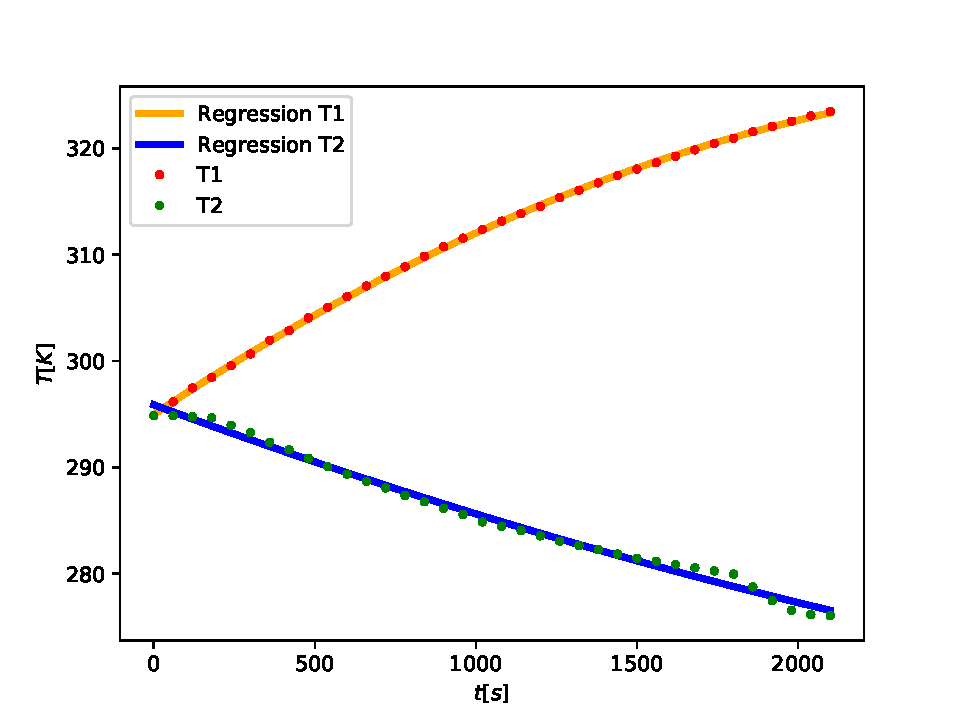
\includegraphics[scale = 0.75]{Temperaturverlaeufe.pdf}
    \caption{Die beiden Temperaturverläufe der Reservoire 1 und 2.}
    \label{fig:TemperaturverlaufA}
  \end{figure}
\section{Aufgabenteil b)}
  Man versuche mit Hilfe einer nicht-linearen Ausgleichsrechnung die gemessenen Temperaturverläufe durch einfache Gleichungen zu approximieren.
  \\
  Die Ausgleichsgleichungen sind ebenfalls in \ref{fig:TemperaturverlaufA} skizziert. Der gewählte Ansatz ist
  \begin{equation}
    T(t) = \symup{A} \cdot t^2 + \symup{B} \cdot t + \symup{C}.
    \label{eq:Regressionsgleichung}
  \end{equation}
  Hierbei ist
\end{document}
